% !TEX root=../root.tex

\subsection{Landing Vehicle}
As flight tests were conducted in a small indoor environement, the landing
vehicle was scaled down in an attempt to better extend to outdoor scenarios. A
landing vehicle was assembled as pictured in~\figref{fig:landing_vehicle}.
During the experiments, the landing vehicle was manually driven around the
motion capture room, following the perimeter of the room and turning at each
wall.

\begin{figure}
  \centering
  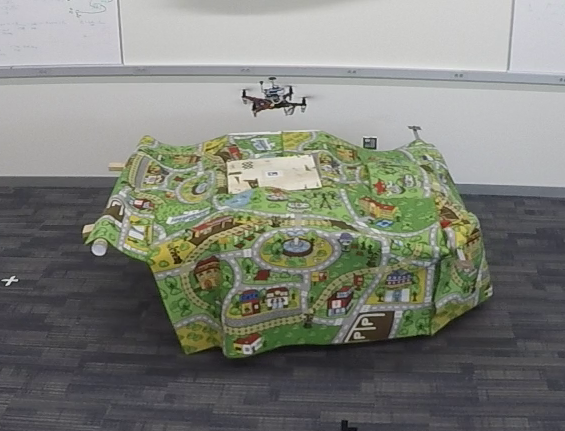
\includegraphics[scale=0.5]{imgs/landing_vehicle.png}
  \caption{Multirotor UAV shown in autonomous flight, tracking the landing
  vehicle.}
  \label{fig:landing_vehicle}
\end{figure}
